\documentclass[12pt,a4paper]{article}
\usepackage[utf8]{vietnam}
\usepackage{amsmath,amssymb}
\usepackage{tabularx}
\usepackage{tikz}
\usetikzlibrary{calc,angles,quotes,arrows.meta,patterns}
\usepackage{xcolor}
\usepackage{enumitem}
\usepackage{fancyhdr}
\usepackage{graphicx}
\usepackage[top=0.9cm, bottom=0.9cm, left=1.2cm, right=1.2cm]{geometry}
\usepackage[loigiai]{ex_test}
\SAOPTN{widthSA=3.2,heightSA=0.62}

\setlength{\headheight}{15pt}
\setlength{\parskip}{0pt}

\pagestyle{fancy}
\fancyhf{}
\rhead{\textit{Môn Toán 8 -- Hướng dẫn giải Đề số 01}}
\lhead{\textit{Bộ đề ôn tập Giữa học kì I}}
\cfoot{\thepage}

\begin{document}

\begin{center}
  \textbf{\Large HƯỚNG DẪN GIẢI CHI TIẾT VÀ BẢNG ĐÁP ÁN}\\
  \textbf{\large ĐỀ ÔN TẬP GIỮA HỌC KỲ I -- ĐỀ SỐ 01}\\
  \textit{Môn: Toán 8 -- Năm học 2026 -- 2027}
\end{center}
\vspace{2mm}

% --- BẢNG ĐÁP ÁN TRẮC NGHIỆM TÓM TẮT ---
\noindent\textbf{\large A. BẢNG ĐÁP ÁN TRẮC NGHIỆM TỔNG HỢP}
\vspace{1mm}

\noindent\textbf{1. Phần I (Mỗi câu trả lời đúng được 0,25 điểm):}
\begin{center}
\begin{tabular}{|c|c|c|c|c|c|c|c|c|c|c|c|c|}
\hline
\textbf{Câu} & \textbf{1} & \textbf{2} & \textbf{3} & \textbf{4} & \textbf{5} & \textbf{6} & \textbf{7} & \textbf{8} & \textbf{9} & \textbf{10} & \textbf{11} & \textbf{12} \\
\hline
\textbf{Đ/A} & \textbf{A} & \textbf{B} & \textbf{D} & \textbf{B} & \textbf{A} & \textbf{B} & \textbf{B} & \textbf{A} & \textbf{A} & \textbf{C} & \textbf{D} & \textbf{D} \\
\hline
\end{tabular}
\end{center}
\vspace{0.5mm}

\noindent\textbf{2. Phần II (Đúng 1 ý: 0,1đ; 2 ý: 0,25đ; 3 ý: 0,5đ; 4 ý: 1,0đ):}
\begin{center}
\begin{tabular}{|c|c|c|c|c||c|c|c|c|c|}
\hline
\textbf{Câu} & \textbf{a)} & \textbf{b)} & \textbf{c)} & \textbf{d)} & \textbf{Câu} & \textbf{a)} & \textbf{b)} & \textbf{c)} & \textbf{d)} \\
\hline
\textbf{Câu 1} & \textbf{Đ} & \textbf{Đ} & \textbf{S} & \textbf{Đ} & \textbf{Câu 2} & \textbf{Đ} & \textbf{Đ} & \textbf{Đ} & \textbf{S} \\
\hline
\end{tabular}
\end{center}
\vspace{0.5mm}

\noindent\textbf{3. Phần III (Mỗi câu trả lời đúng được 1,0 điểm):}
\begin{center}
\begin{tabular}{|c|c|c|}
\hline
\textbf{Câu} & \textbf{Câu 1} & \textbf{Câu 2} \\
\hline
\textbf{Đáp án} & $\mathbf{3x^2y + 3}$ & $\mathbf{6x + 18}$ \\
\hline
\end{tabular}
\end{center}
\vspace{1.5mm}

% --- B. LỜI GIẢI CHI TIẾT ---
\noindent\textbf{\large B. LỜI GIẢI CHI TIẾT CÁC CÂU HỎI}
\vspace{1mm}

\noindent\textbf{\large PHẦN I. CÂU TRẮC NGHIỆM NHIỀU PHƯƠNG ÁN LỰA CHỌN}
\vspace{1mm}
\begin{ex}
Biểu thức nào sau đây là đơn thức?
\choice
{\True $5x^2y$}
{$2xy + 1$}
{$3x - 2$}
{$x^2 + 7$}
\loigiai{
Đơn thức là biểu thức đại số chỉ gồm một số, một biến, hoặc một tích giữa các số và các biến. Do đó $5x^2y$ là đơn thức; các biểu thức còn lại đều là đa thức chứa phép cộng hoặc trừ.
}
\end{ex}

\begin{ex}
Đơn thức đồng dạng với đơn thức $5x^3yz$ là:
\choice
{$-30x^2yz$}
{\True $x^3yz$}
{$-30xyz$}
{$40x^3y^5z$}
\loigiai{
Hai đơn thức đồng dạng là hai đơn thức có hệ số khác 0 và có cùng phần biến. Đơn thức $x^3yz$ có cùng phần biến $x^3yz$ với đơn thức đã cho.
}
\end{ex}

\begin{ex}
Bậc của đa thức $A = 5x^3yz + \dfrac{1}{2}xy - 0{,}5x^4y^2$ là:
\choice
{3}
{4}
{5}
{\True 6}
\loigiai{
Ta xác định bậc của từng hạng tử trong đa thức:
- Hạng tử $5x^3yz$ có bậc là $3 + 1 + 1 = 5$.
- Hạng tử $\dfrac{1}{2}xy$ có bậc là $1 + 1 = 2$.
- Hạng tử $-0{,}5x^4y^2$ có bậc là $4 + 2 = 6$.
Bậc của đa thức là bậc của hạng tử có bậc cao nhất, tức là 6.
}
\end{ex}

\begin{ex}
Cho hình chóp tam giác đều $A.BCD$ như hình vẽ bên. Đoạn thẳng nào sau đây là trung đoạn của hình chóp?
\begin{center}
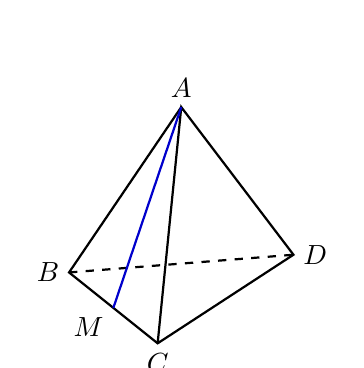
\begin{tikzpicture}[scale=0.75, baseline=(current bounding box.center)]
  \coordinate (B) at (0,0);
  \coordinate (D) at (3.8,0.3);
  \coordinate (C) at (1.5,-1.2);
  \coordinate (A) at (1.9,2.8);
  \coordinate (M) at ($(B)!0.5!(C)$);
  \draw[thick] (A) -- (B) -- (C) -- (D) -- (A) -- (C);
  \draw[dashed, thick] (B) -- (D);
  \draw[thick, blue!80!black] (A) -- (M);
  \node[above] at (A) {$A$};
  \node[left] at (B) {$B$};
  \node[below] at (C) {$C$};
  \node[right] at (D) {$D$};
  \node[below left] at (M) {$M$};
\end{tikzpicture}
\end{center}
\choice
{$AC$}
{\True $AM$}
{$BN$}
{$AP$}
\loigiai{
Trung đoạn của hình chóp đều là đường cao vẽ từ đỉnh của mặt bên xuống cạnh đáy tương ứng. Trong hình vẽ, đoạn thẳng $AM$ vuông góc với cạnh đáy $BC$ tại trung điểm $M$ của $BC$, do đó $AM$ là trung đoạn của hình chóp.
}
\end{ex}

\begin{ex}
Tổng các góc của một tứ giác lồi bằng:
\choice
{\True $360^\circ$}
{$180^\circ$}
{$270^\circ$}
{$120^\circ$}
\loigiai{
Theo định lý về tổng các góc trong một tứ giác, tổng số đo 4 góc của một tứ giác luôn bằng $360^\circ$.
}
\end{ex}

\begin{ex}
Giá trị của biểu thức $x^3 - 3x^2 + 3x - 1$ tại $x = 2$ là:
\choice
{0}
{\True 1}
{2}
{16}
\loigiai{
Ta nhận thấy hằng đẳng thức lập phương của một hiệu:
$$x^3 - 3x^2 + 3x - 1 = (x - 1)^3.$$
Thay $x = 2$ vào biểu thức, ta được: $(2 - 1)^3 = 1^3 = 1$.
}
\end{ex}

\begin{ex}
Kết quả của phép tính $\dfrac{a - 2}{a - b} - \dfrac{2 - b}{b - a}$ là:
\choice
{$-1$}
{\True 1}
{$\dfrac{a - b}{b - a}$}
{$\dfrac{a + b - 4}{a - b}$}
\loigiai{
Đổi dấu phân thức thứ hai:
$$\dfrac{a - 2}{a - b} - \dfrac{2 - b}{b - a} = \dfrac{a - 2}{a - b} + \dfrac{2 - b}{a - b} = \dfrac{(a - 2) + (2 - b)}{a - b} = \dfrac{a - b}{a - b} = 1.$$
}
\end{ex}

\begin{ex}
Cho tam giác $ABC$ vuông tại $A$ có $AB = 3\text{ cm}, AC = 4\text{ cm}$. Độ dài cạnh $BC$ bằng:
\choice
{\True $5\text{ cm}$}
{$6\text{ cm}$}
{$7\text{ cm}$}
{$8\text{ cm}$}
\loigiai{
Áp dụng định lý Pythagoras cho tam giác $ABC$ vuông tại $A$:
$$BC^2 = AB^2 + AC^2 = 3^2 + 4^2 = 9 + 16 = 25 \Rightarrow BC = \sqrt{25} = 5\text{ cm}.$$
}
\end{ex}

\begin{ex}
Hình chữ nhật là tứ giác có:
\choice
{\True 4 góc vuông}
{2 góc kề một cạnh bằng nhau}
{2 góc kề một cạnh cùng bằng $90^\circ$}
{2 góc kề một cạnh bù nhau}
\loigiai{
Theo định nghĩa chuẩn, hình chữ nhật là tứ giác có bốn góc vuông.
}
\end{ex}

\begin{ex}
Hình bình hành có hai cạnh kề bằng nhau là hình gì?
\choice
{Hình chữ nhật}
{Hình vuông}
{\True Hình thoi}
{Hình thang}
\loigiai{
Theo dấu hiệu nhận biết các tứ giác, hình bình hành có hai cạnh kề bằng nhau là hình thoi.
}
\end{ex}

\begin{ex}
Cho hình thang cân $ABCD$ có $AB \parallel CD$ và $\widehat{A} = 125^\circ$. Số đo của $\widehat{C}$ là:
\choice
{$125^\circ$}
{$65^\circ$}
{$90^\circ$}
{\True $55^\circ$}
\loigiai{
Do $AB \parallel CD$ nên $\widehat{A} + \widehat{D} = 180^\circ$ (hai góc trong cùng phía bù nhau).
Suy ra: $\widehat{D} = 180^\circ - 125^\circ = 55^\circ$.
Do $ABCD$ là hình thang cân nên hai góc kề đáy bằng nhau: $\widehat{C} = \widehat{D} = 55^\circ$.
}
\end{ex}

\begin{ex}
Tìm khẳng định sai trong các khẳng định sau:
\choice
{Hình chữ nhật có hai cạnh kề bằng nhau là hình vuông}
{Hình chữ nhật có hai đường chéo vuông góc là hình vuông}
{Hình chữ nhật có một đường chéo là đường phân giác của một góc vuông là hình vuông}
{\True Hình chữ nhật có bốn góc vuông là hình vuông}
\loigiai{
Khẳng định D sai vì bản thân mọi hình chữ nhật đều có 4 góc vuông theo định nghĩa, điều này không đủ để biến nó thành hình vuông (hình vuông cần thêm điều kiện 4 cạnh bằng nhau hoặc 2 đường chéo vuông góc).
}
\end{ex}


\setcounter{ex}{0}
\noindent\textbf{\large PHẦN II. CÂU TRẮC NGHIỆM ĐÚNG SAI}
\vspace{1mm}
\begin{ex}
Cho hai đa thức $A = 3x^2y - 2xy^2 + 5$ và $B = x^2y + xy^2 - 1$. Xét tính đúng sai của các mệnh đề sau:
\choiceTF
{\True Bậc của đa thức $A$ bằng 3}
{\True Tổng của hai đa thức là $A + B = 4x^2y - xy^2 + 4$}
{Tại $x = 1$ và $y = -1$, giá trị của đa thức $B$ bằng 1}
{\True Tích của đa thức $A$ với đơn thức $2xy$ là $6x^3y^2 - 4x^2y^3 + 10xy$}
\loigiai{
\textbf{a)} Đúng. Đa thức $A$ gồm các hạng tử có bậc lần lượt là 3, 3 và 0; do đó bậc cao nhất là 3.

\textbf{b)} Đúng. $A + B = (3x^2y + x^2y) + (-2xy^2 + xy^2) + (5 - 1) = 4x^2y - xy^2 + 4$.

\textbf{c)} Sai. Thay $x = 1, y = -1$ vào $B$: $B = 1^2 \cdot (-1) + 1 \cdot (-1)^2 - 1 = -1 + 1 - 1 = -1 \ne 1$.

\textbf{d)} Đúng. $A \cdot 2xy = (3x^2y - 2xy^2 + 5) \cdot 2xy = 6x^3y^2 - 4x^2y^3 + 10xy$.
}
\end{ex}

\begin{ex}
Cho biểu thức $P = (x + 3)^2 - (x - 3)(x + 3)$ và đa thức $Q = x^3 - 4x$. Xét tính đúng sai của các mệnh đề sau:
\choiceTF
{\True Khai triển hằng đẳng thức $(x + 3)^2$ ta được $x^2 + 6x + 9$}
{\True Kết quả rút gọn của biểu thức $P$ là $6x + 18$}
{\True Phân tích đa thức $Q$ thành nhân tử ta được $x(x - 2)(x + 2)$}
{Tại $x = -3$, giá trị của biểu thức $P$ bằng 12}
\loigiai{
\textbf{a)} Đúng. Áp dụng $(a+b)^2 = a^2 + 2ab + b^2$, ta có $(x+3)^2 = x^2 + 6x + 9$.

\textbf{b)} Đúng. $P = (x^2 + 6x + 9) - (x^2 - 9) = x^2 + 6x + 9 - x^2 + 9 = 6x + 18$.

\textbf{c)} Đúng. $Q = x(x^2 - 4) = x(x - 2)(x + 2)$.

\textbf{d)} Sai. Thay $x = -3$ vào $P$: $P = 6 \cdot (-3) + 18 = -18 + 18 = 0 \ne 12$.
}
\end{ex}


\setcounter{ex}{0}
\noindent\textbf{\large PHẦN III. CÂU HỎI TRẢ LỜI NGẮN}
\vspace{1mm}
\begin{ex}
Cho hai đa thức $A = 2x^2y - 3xy + 5$ và $B = x^2y + 3xy - 2$. Tính $A + B$. \shortans{$3x^2y + 3$}
\loigiai{
Thực hiện phép cộng hai đa thức:
$$\begin{aligned} A + B &= (2x^2y - 3xy + 5) + (x^2y + 3xy - 2) \\ &= (2x^2y + x^2y) + (-3xy + 3xy) + (5 - 2) \\ &= 3x^2y + 3. \end{aligned}$$
Đáp số: $3x^2y + 3$.
}
\end{ex}

\begin{ex}
Rút gọn biểu thức $P = (x + 3)^2 - (x - 3)(x + 3)$. \shortans{$6x + 18$}
\loigiai{
Áp dụng các hằng đẳng thức đáng nhớ:
- $(x + 3)^2 = x^2 + 6x + 9$
- $(x - 3)(x + 3) = x^2 - 9$
Khi đó:
$$P = (x^2 + 6x + 9) - (x^2 - 9) = x^2 + 6x + 9 - x^2 + 9 = 6x + 18.$$
Đáp số: $6x + 18$.
}
\end{ex}


\setcounter{ex}{0}
\noindent\textbf{\large PHẦN IV. TỰ LUẬN (HƯỚNG DẪN GIẢI VÀ THANG ĐIỂM)}
\vspace{1mm}
\begin{ex} (2,0 điểm)
Thực hiện phép tính:
\begin{enumerate}[label=\textbf{\alph*)}, leftmargin=0.8cm, itemsep=0pt, topsep=1pt]
\item (0,5 điểm) $xy(x + y)$
\item (0,5 điểm) $(x - 2)^2 + 2x(x - 6)$
\item (1,0 điểm) $(2x^2 - 5xy - 4y^2)x - (2x^4y - 3x^3y^2 + 4x^2y^3) : xy$
\end{enumerate}
\loigiai{
\textbf{a)} \textit (0,5 điểm): $xy(x + y) = xy \cdot x + xy \cdot y = x^2y + xy^2$.

\textbf{b)} \textit (0,5 điểm): $\begin{aligned}[t] (x - 2)^2 + 2x(x - 6) &= (x^2 - 4x + 4) + (2x^2 - 12x) \\ &= 3x^2 - 16x + 4. \end{aligned}$

\textbf{c)} \textit (1,0 điểm): $\begin{aligned}[t] &\quad (2x^2 - 5xy - 4y^2)x - (2x^4y - 3x^3y^2 + 4x^2y^3) : xy \\ &= (2x^3 - 5x^2y - 4xy^2) - (2x^3 - 3x^2y + 4xy^2) \\ &= 2x^3 - 5x^2y - 4xy^2 - 2x^3 + 3x^2y - 4xy^2 \\ &= -2x^2y - 8xy^2. \end{aligned}$


}
\end{ex}
\vspace{0.5mm}

\begin{ex} (1,5 điểm)
Phân tích các đa thức sau thành nhân tử:
\begin{enumerate}[label=\textbf{\alph*)}, leftmargin=0.8cm, itemsep=0pt, topsep=1pt]
\item (0,25 điểm) $4x^2 - 12x$
\item (0,25 điểm) $x^3 - 4x^2 + 4x$
\item (0,5 điểm) $x^2 - y^2 - 5x - 5y$
\item (0,5 điểm) $x^2 + 2xy + y^2 - 16$
\end{enumerate}
\loigiai{
\textbf{a)} \textit (0,25 điểm): $4x^2 - 12x = 4x(x - 3)$.

\textbf{b)} \textit (0,25 điểm): $x^3 - 4x^2 + 4x = x(x^2 - 4x + 4) = x(x - 2)^2$.

\textbf{c)} \textit (0,5 điểm): $\begin{aligned}[t] x^2 - y^2 - 5x - 5y &= (x^2 - y^2) - (5x + 5y) \\ &= (x - y)(x + y) - 5(x + y) \\ &= (x + y)(x - y - 5). \end{aligned}$

\textbf{d)} \textit (0,5 điểm): $\begin{aligned}[t] x^2 + 2xy + y^2 - 16 &= (x + y)^2 - 4^2 \\ &= (x + y - 4)(x + y + 4). \end{aligned}$


}
\end{ex}
\vspace{0.5mm}

\begin{ex} (1,0 điểm)
Cho tam giác $ABC$ vuông tại $A$ ($AB < AC$). Gọi $I$ là trung điểm của $BC$. Qua $I$ vẽ $IM \perp AB$ tại $M$, $IN \perp AC$ tại $N$.
\begin{center}
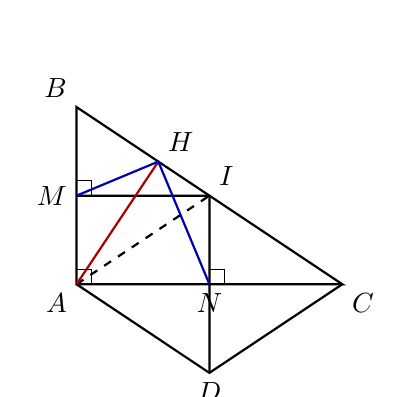
\begin{tikzpicture}[scale=0.75, baseline=(current bounding box.center)]
  \coordinate (A) at (0,0);
  \coordinate (B) at (0,3);
  \coordinate (C) at (4.5,0);
  \coordinate (I) at ($(B)!0.5!(C)$);
  \coordinate (M) at (0,1.5);
  \coordinate (N) at (2.25,0);
  \coordinate (D) at ($(N)!-1!(I)$);
  \coordinate (H) at ($(B)!(A)!(C)$);
  \draw[thick] (A) -- (B) -- (C) -- cycle;
  \draw[thick] (I) -- (M);
  \draw[thick] (I) -- (D);
  \draw[thick] (A) -- (D) -- (C);
  \draw[thick, dashed] (A) -- (I);
  \draw[thick, red!70!black] (A) -- (H);
  \draw[thick, blue!70!black] (M) -- (H) -- (N);
  \draw (0,0.25) -- (0.25,0.25) -- (0.25,0);
  \draw (0,1.75) -- (0.25,1.75) -- (0.25,1.5);
  \draw (2.25,0.25) -- (2.5,0.25) -- (2.5,0);
  \node[below left] at (A) {$A$};
  \node[above left] at (B) {$B$};
  \node[below right] at (C) {$C$};
  \node[above right] at (I) {$I$};
  \node[left] at (M) {$M$};
  \node[below] at (N) {$N$};
  \node[below] at (D) {$D$};
  \node[above right] at (H) {$H$};
\end{tikzpicture}
\end{center}
\begin{enumerate}[label=\textbf{\alph*)}, leftmargin=0.8cm, itemsep=0pt, topsep=1pt]
\item (0,5 điểm) Chứng minh rằng tứ giác $AMIN$ là hình chữ nhật.
\item (0,25 điểm) Lấy điểm $D$ trên tia đối của tia $NI$ sao cho $N$ là trung điểm của $ID$. Chứng minh tứ giác $ADCI$ là hình thoi.
\item (0,25 điểm) Kẻ $AH \perp BC$ tại $H$. Chứng minh $MH \perp HN$.
\end{enumerate}
\loigiai{
\textbf{a)} \textit (0,5 điểm): Xét tứ giác $AMIN$, ta có:
- $\widehat{MAN} = 90^\circ$ (do tam giác $ABC$ vuông tại $A$),
- $\widehat{AMI} = 90^\circ$ (do $IM \perp AB$),
- $\widehat{ANI} = 90^\circ$ (do $IN \perp AC$).
Tứ giác $AMIN$ có 3 góc vuông nên $AMIN$ là hình chữ nhật.

\textbf{b)} \textit (0,25 điểm): Trong tam giác $ABC$, $I$ là trung điểm $BC$ và $IN \parallel AB$ (cùng vuông góc với $AC$), suy ra $N$ là trung điểm của $AC$.
Tứ giác $ADCI$ có hai đường chéo $AC$ và $ID$ cắt nhau tại trung điểm $N$ của mỗi đường, nên $ADCI$ là hình bình hành.
Mặt khác, $AC \perp ID$ tại $N$ (vì $IN \perp AC$).
Hình bình hành $ADCI$ có hai đường chéo vuông góc nên $ADCI$ là hình thoi.

\textbf{c)} \textit (0,25 điểm): Vì $AMIN$ là hình chữ nhật nên 4 điểm $A, M, I, N$ cùng nằm trên đường tròn đường kính $AI$.
Xét tam giác $AHI$ vuông tại $H$ ($AH \perp BC$), điểm $H$ cũng nằm trên đường tròn đường kính $AI$.
Do đó 5 điểm $A, M, H, I, N$ cùng nằm trên đường tròn đường kính $AI$, hay cũng chính là đường tròn đường kính $MN$ (vì trong hình chữ nhật $AMIN$, $AI = MN$).
Điểm $H$ nhìn đoạn $MN$ dưới một góc vuông, suy ra $\widehat{MHN} = 90^\circ$, hay $MH \perp HN$.


}
\end{ex}
\vspace{0.5mm}

\begin{ex} (0,5 điểm)
Cho các số thực $x, y$ thỏa mãn điều kiện:
$$2x^2 + 10y^2 - 6xy - 6x - 2y + 10 = 0.$$
Tính giá trị của biểu thức $A = \dfrac{(x + y - 4)^{2018} - y^{2018}}{x}$.
\begin{enumerate}[label=\textbf{\alph*)}, leftmargin=0.8cm, itemsep=0pt, topsep=1pt]
\item (0,5 điểm) Tính giá trị biểu thức $A$.
\end{enumerate}
\loigiai{
\textbf{a)} \textit (0,5 điểm): Biến đổi phương trình ban đầu thành tổng các bình phương:
$$\begin{aligned} &\quad 2x^2 + 10y^2 - 6xy - 6x - 2y + 10 = 0 \\ &\Leftrightarrow (x^2 - 6xy + 9y^2) + (x^2 - 6x + 9) + (y^2 - 2y + 1) = 0 \\ &\Leftrightarrow (x - 3y)^2 + (x - 3)^2 + (y - 1)^2 = 0. \end{aligned}$$
Vì $(x - 3y)^2 \ge 0$, $(x - 3)^2 \ge 0$, $(y - 1)^2 \ge 0$ với mọi $x, y$.
Do đó đẳng thức xảy ra khi và chỉ khi:
$$\begin{cases} x - 3y = 0 \\ x - 3 = 0 \\ y - 1 = 0 \end{cases} \Leftrightarrow \begin{cases} x = 3 \\ y = 1. \end{cases}$$
Thay $x = 3, y = 1$ vào biểu thức $A$, ta được:
$$A = \dfrac{(3 + 1 - 4)^{2018} - 1^{2018}}{3} = \dfrac{0^{2018} - 1}{3} = -\dfrac{1}{3}.$$
Vậy $A = -\dfrac{1}{3}$.


}
\end{ex}
\vspace{0.5mm}


\enlargethispage{1.5cm}
\begin{center}
\rule{4cm}{0.4pt}\\
\textit{--- HẾT ---}
\end{center}
\end{document}
